\appendix 

\begin{figure} [hb!]
\centering
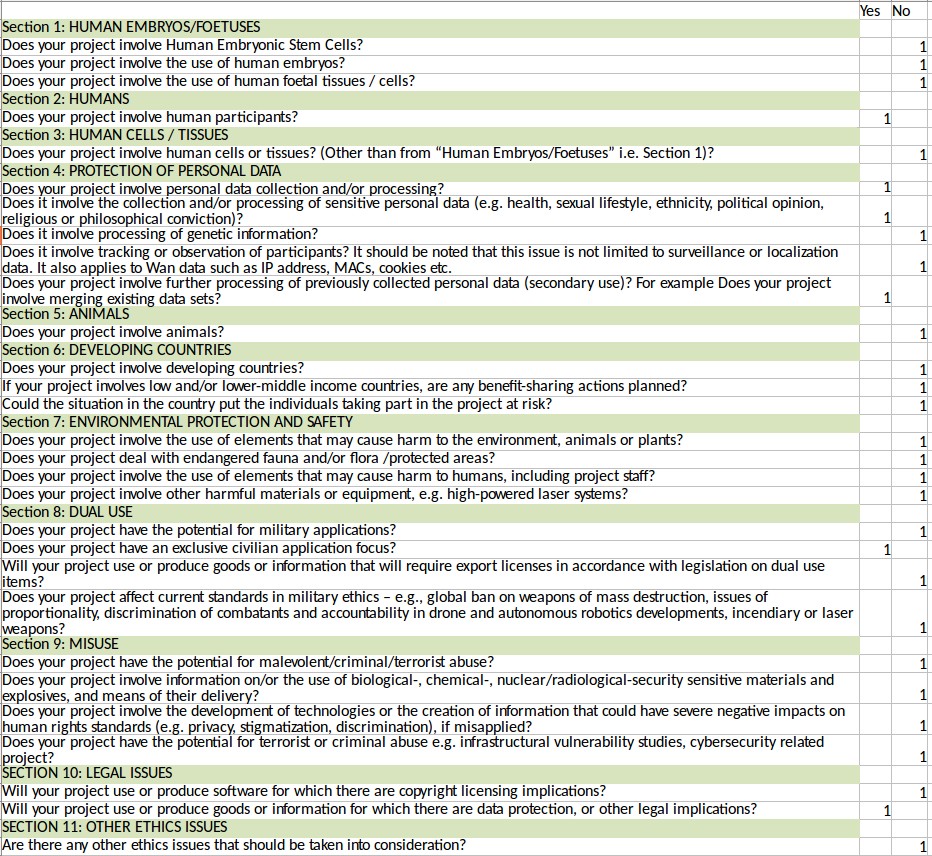
\includegraphics[scale=0.5]{pictures/ethics2}
\caption{Ethics checklist}
\label{fig:ethics}
\end{figure}

\section{Ethics}
I have filled out a table of standard ethical questions (shown in figure \ref{fig:ethics}). My project makes no direct use of stem cells or any other questionable material. In order to use my website, individuals will need to upload medical imagery (sensitive material) to a server, so that the CNN may learn. In the full product, the data would be uploaded over a secure connection (TLS) to protect the privacy of the patients. Medical data can now be anonymized fairly effectively. The user has the option of uploading the image or not, so this would only be done if the image was properly anonymized. If the user does not upload the image, then it is only ever held in RAM by the segmentation algorithm and is therefore destroyed once the segmentation has been performed.

Other than that, the project has exclusively civilian applications and is generally ethically positive as a device to aid in healthcare.



